\documentclass[10pt,a4paper]{article}

\usepackage[T1]{fontenc}
\usepackage[polish]{babel}
\usepackage[utf8]{inputenc}
\usepackage{graphicx}
\usepackage[export]{adjustbox}

\graphicspath{ {./../media/} }

\usepackage[margin=1.2in]{geometry}

\usepackage{hyperref}
\hypersetup{
    colorlinks=true,
    linkcolor=black,
    filecolor=magenta,      
    urlcolor=blue,
}

\usepackage{amsfonts}
\usepackage{titlesec}

\titleformat{\chapter}[hang] 
{\normalfont\huge\bfseries}{\chaptertitlename\ \thechapter:}{1em}{} 
\titleformat*{\section}{\huge}
\begin{document}

\title{\Huge Instalacja Arch Linux}
\author{Maciej Tracz \\\\Technikum Mechatroniczne nr 1 w Warszawie}
\date{Rok 2020}
\maketitle

\section{Instalacja}
	
Proces instalowania warto podzielić na 3 etapy:
\begin{enumerate}
\item Tworzenie nośnika ISO
\item Instalacja systemu na docelowej maszynie
\item Konfiguracja poinstalacyjna\\
\end{enumerate}	
Teraz kolejno przejdziemy przez wszystkie 3 na przykładzie Linux Manjaro XFCE 20.0.3.
		\subsection{Tworzenie nośnika}
Aby móc zainstalować system operacyjny na komputerze potrzebujemy urządzenia będącego nośnikiem obrazu takiego systemu. Do tego potrzebujemy pendriva conajmniej 8GB oraz obrazu systemu w postaci ISO. Taki można pobrać na stronach twórców w zakładce Downloads. Gdy mamy już te elementy potrzebujemy narzędzia, które przygotuje pendriva jako nośnik. Polecam Rufusa dla użytkowników Windowsa oraz UUByte Software na MacOS. Nie są to jednak jedyne opcje i warto poszukać czy aktualnie nie wyszły nowsze, lepsze narzędzia.\\\\Windows\\\\Rufus: \url{https://rufus.ie/}\\ YUMI: \url{https://www.pendrivelinux.com/yumi-multiboot-usb-creator/}\\\\MacOS\\\\\ UUByte Software: \url{https://www.uubyte.com/download/uubyte-iso-editor.dmg}\\Disk Utility - The Default ISO Buner (narzędzie wbudowane, polecane na starych urządzeniach.)\\\\\\ Teraz gdy masz masz wszytsko co potrzebne, postępuj zgodnie z instrukcją na stronie lub po prostu dodaj ISO i wybierz domyślne ustawienia. Jeśli posiadasz już odpowiednio przygotowanego pendriva przejdzmy do następnego etapu.

\newpage

\section{Instalacja\\}

\begin{enumerate}

\item Wybór urządzenia rozruchowego\\\\
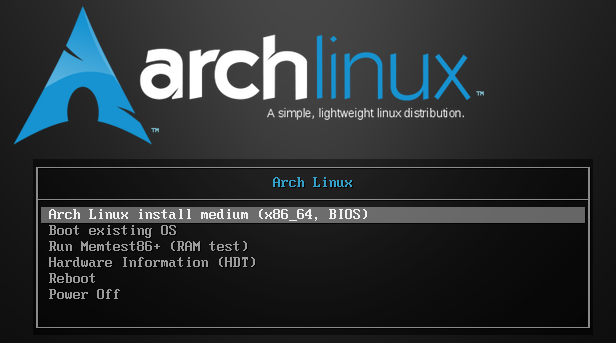
\includegraphics[width=0.8\textwidth, center]{arch1.png}\\\\
\item Uruchomienie środwiska instalacyjnego Live\\\\
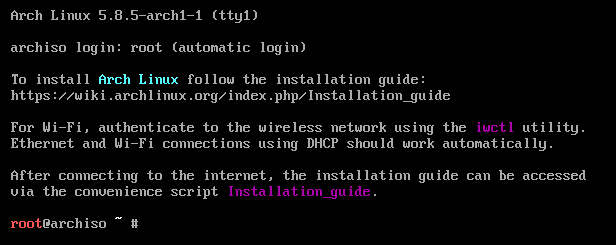
\includegraphics[width=0.8\textwidth, center]{arch2.png}
\newpage
\item Partycjonowanie dysku Root\\\\
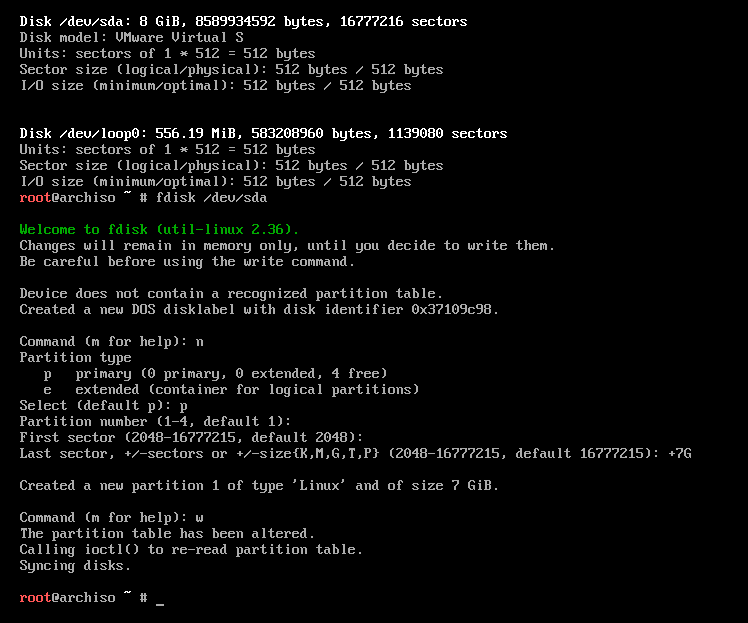
\includegraphics[width=0.8\textwidth, center]{arch3.png}\\\\
\item Partycjonownanie przestrzeni wymiany\\\\
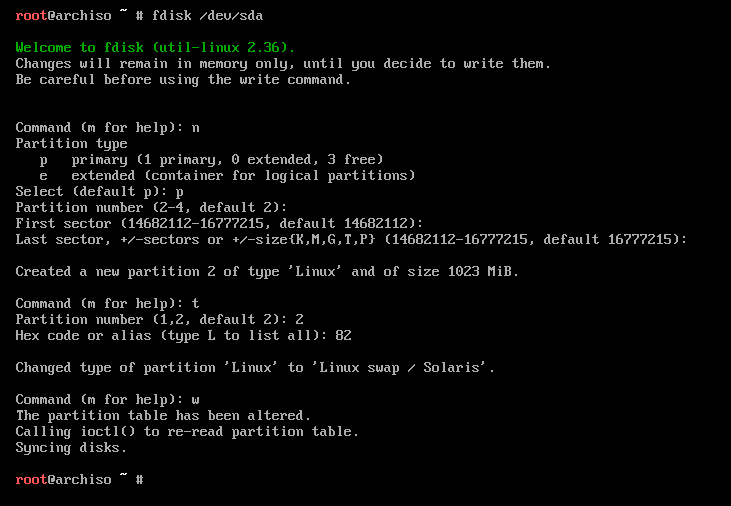
\includegraphics[width=0.8\textwidth, center]{arch4.png}\\\\
\newpage
\item Sprawdzanie wykonania operacji na dyskach\\\\
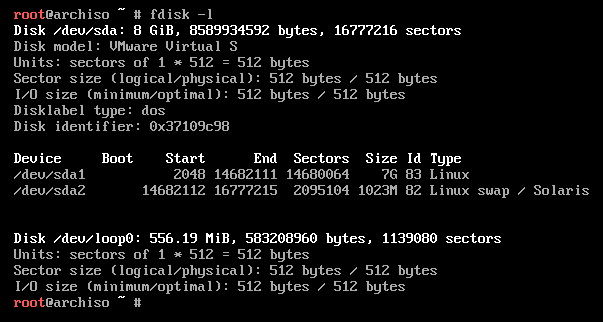
\includegraphics[width=0.8\textwidth, center]{arch5.png}\\\\
\item Formatowanie partycji Root systemem plików ext4\\\\
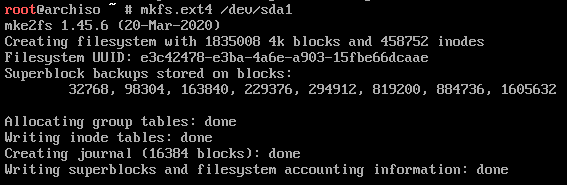
\includegraphics[width=0.8\textwidth, center]{arch6.png}\\\\
\item Nawiązanie połączenia z internetem (w przypadku wifi użyj komendy wifi-menu)\\\\
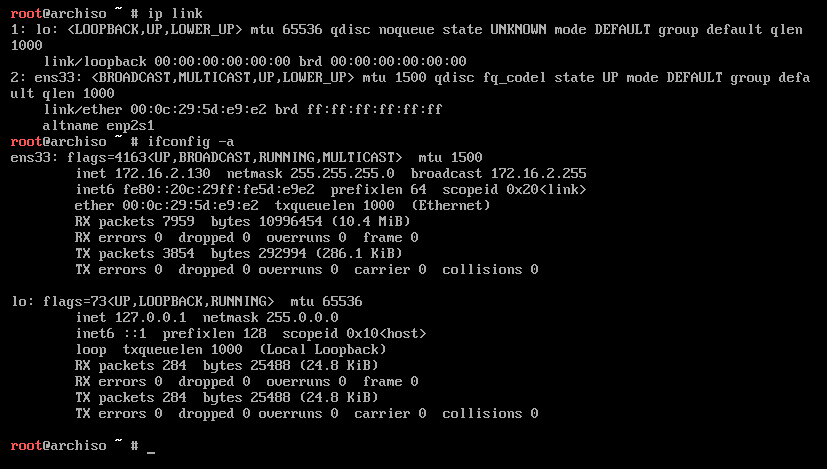
\includegraphics[width=0.8\textwidth, center]{arch7.png}\\\\
\newpage
\item Pozyskanie list źródeł pakietów\\\\
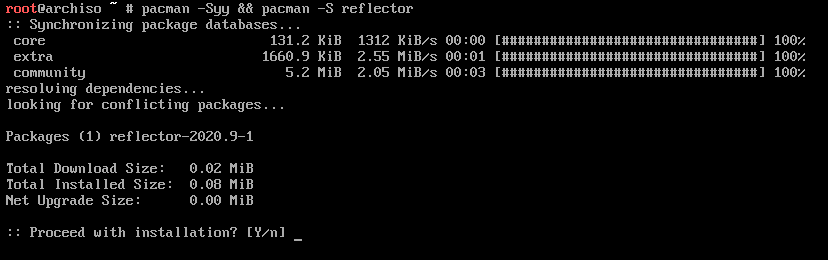
\includegraphics[width=0.8\textwidth, center]{arch8.png}\\\\
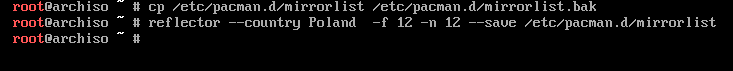
\includegraphics[width=0.8\textwidth, center]{arch9.png}\\\\
\item Zainstaluj Archa \\\\
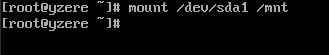
\includegraphics[width=0.8\textwidth, center]{arch10-1.png}\\\\
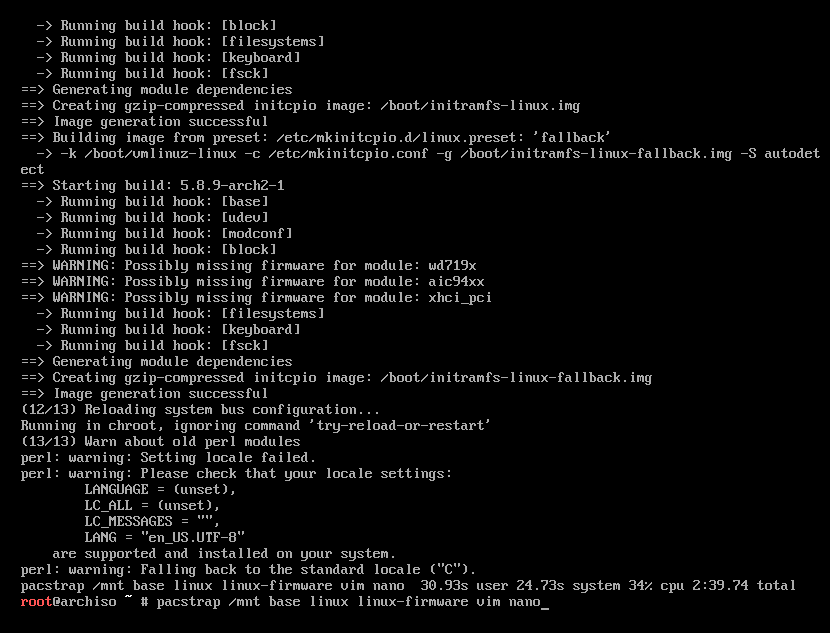
\includegraphics[width=1\textwidth, center]{arch10.png}\\\\
\newpage
\item Konfiguracja 
\begin{itemize}
\item  Wygenerowanie fstab i dodanie strefy czasowej\\\\
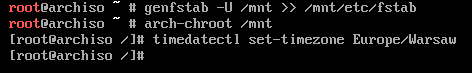
\includegraphics[width=0.8\textwidth, center]{arch11.png}\\\\
\item  Dodanie naszego konta do hostów i stworzenie pliku locale\\\\
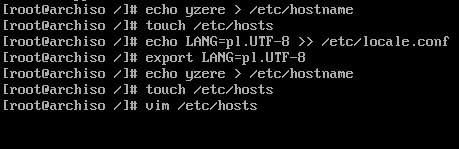
\includegraphics[width=0.8\textwidth, center]{arch12.png}\\\\
\item Ustawienie adresów sieciowych na maszynie\\\\
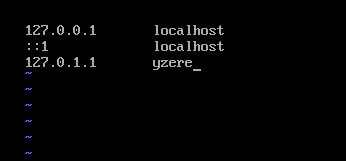
\includegraphics[width=0.8\textwidth, center]{arch13.png}\\\\
\item Ustawianie hasła do konta root\\\\
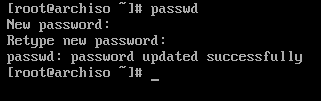
\includegraphics[width=0.8\textwidth, center]{arch14.png}\\\\

\end{itemize}
\newpage
\item Instalacja bootloadera Grub\\\\
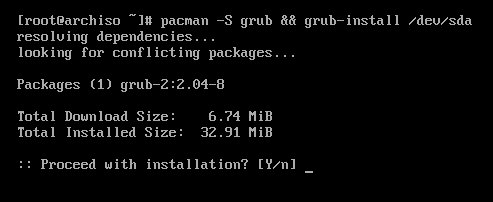
\includegraphics[width=0.8\textwidth, center]{arch15.png}\\\\
\item Generowanie pliku konfiguracyjnego Grub-a\\\\
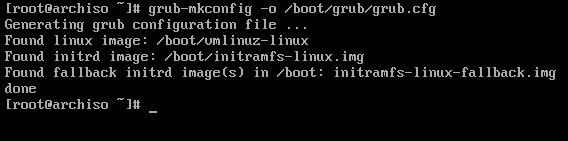
\includegraphics[width=0.8\textwidth, center]{arch16.png}\\\\
\item Teraz wpisz 'exit' (może 2 razy z rzędu), a po tym 'shutdown now' / 'reboot now'. Twój system jest gotowy do używania. Naciesz się terminalem :)

\end{enumerate}


\end{document}